\documentclass[aspectratio=169, lualatex, handout]{beamer}
\makeatletter\def\input@path{{theme/}}\makeatother\usetheme{cipher}

\title{Applied Cryptography - 2.7: Cryptocurrency Cryptography}
\author{Nadim Kobeissi}
\subject{An exploration of cryptocurrency cryptography, covering Bitcoin's proof-of-work consensus mechanism, transaction structures, and Ethereum's smart contract platform.}
\keywords{Bitcoin, Proof-of-Work, Blockchain, Consensus, Double-Spending, Merkle Trees, UTXO, Mining, Ethereum, Smart Contracts, EVM, Gas}
\institute{American University of Beirut}
\instituteimage{images/aub-white.png}
\date{\today}
\coversubtitle{CMPS 297AD/396AI\\Fall 2025}
\coverpartname{Part 2: Real-World Cryptography}
\covertopicname{2.7: Cryptocurrency Cryptography}
\coverwebsite{https://appliedcryptography.page}

\begin{document}
\begin{frame}[plain]
	\titlepage
\end{frame}

\section{Bitcoin}

\begin{frame}{The problem: trust in digital commerce}
	\begin{itemize}
		\item Online commerce relies entirely on financial institutions as trusted third parties.
		\item Banks, payment processors, credit card companies mediate every transaction.
		\item This trust-based model has fundamental limitations:
		      \begin{itemize}
			      \item Intrinsic dependence on centralized parties.
			      \item Financial institutions must mediate disputes.
			      \item Increases transaction costs significantly.
		      \end{itemize}
	\end{itemize}
\end{frame}

\begin{frame}{Weaknesses of the trust-based model}
	\begin{itemize}
		\item \textbf{High transaction costs}: Mediation costs make micropayments impractical.
		\item \textbf{Reversibility spreads distrust}: Merchants need extensive customer information.
		\item \textbf{Fraud is inevitable}: Some percentage of fraud accepted as cost of business.
		\item \textbf{No digital cash equivalent}: Physical cash works person-to-person, but no digital. analog exists
	\end{itemize}
\end{frame}

\begin{frame}{Peer-to-peer electronic cash}
	\begin{itemize}
		\item Replace trust with cryptographic proof.
		\item Enable direct transactions between parties without intermediaries.
		\item Key properties needed:
		      \begin{itemize}
			      \item Computationally impractical to reverse (protects sellers).
			      \item Optional escrow mechanisms (protects buyers).
			      \item No reliance on third parties.
		      \end{itemize}
	\end{itemize}
\end{frame}

\begin{frame}{Core challenge: double spending}
	\begin{itemize}
		\item Digital information can be copied perfectly.
		\item Without a central authority, how do we prevent spending the same coin twice?
		\item Traditional solution: Central mint/bank tracks all transactions.
		\item Problem: This reintroduces the trusted third party.
	\end{itemize}
\end{frame}

\begin{frame}{Bitcoin's solution}
	\begin{itemize}
		\item Peer-to-peer distributed timestamp server.
		\item Generates computational proof of transaction order.
		\item Security assumption: Honest nodes control majority of CPU power.
		\item Key innovations:
		      \begin{itemize}
			      \item Proof-of-work consensus mechanism.
			      \item Blockchain as public ledger.
			      \item Economic incentives for honest behavior.
		      \end{itemize}
	\end{itemize}
\end{frame}

\begin{frame}{Historical context}
	\begin{itemize}
		\item Published October 31, 2008 by Satoshi Nakamoto (pseudonym)
		\item Built on decades of cryptographic research:
		      \begin{itemize}
			      \item Digital signatures (ECDSA)
			      \item Hashcash proof-of-work (Adam Back, 1997)
			      \item Cryptographic timestamps (Haber \& Stornetta, 1991)
			      \item B-money and bit gold proposals (Wei Dai, Nick Szabo)
		      \end{itemize}
		\item First practical solution to Byzantine Generals Problem for money.
	\end{itemize}
\end{frame}

\begin{frame}{The Byzantine Generals Problem}
	\begin{itemize}
		\item Classical problem in distributed computing (Lamport, Shostak, Pease, 1982).
		\item Scenario: Byzantine generals must coordinate attack on a city.
		      \begin{itemize}
			      \item Generals can only communicate via messengers.
			      \item Some generals may be traitors sending false messages.
			      \item Need consensus: all loyal generals execute same plan.
		      \end{itemize}
		\item Core challenge: How to achieve reliable consensus when:
		      \begin{itemize}
			      \item Communication channels are unreliable.
			      \item Some participants may be malicious.
			      \item No central authority to trust.
		      \end{itemize}
		\item \textbf{Bitcoin's breakthrough}: First practical solution for digital money using proof-of-work.
	\end{itemize}
\end{frame}

\subsection{Blockchains}

\begin{frame}{Let's start with the basics: What's a blockchain?}
	\begin{columns}[c]
		\begin{column}{0.5\textwidth}
			\textbf{Think of it like a notebook:}
			\begin{itemize}
				\item Pages = blocks
				\item Each page lists transactions
				\item Pages linked together in order
				\item Can't tear out or reorder pages
			\end{itemize}
			\vspace{0.5em}
			\textbf{But it's distributed:}
			\begin{itemize}
				\item Everyone has a copy
				\item No single owner
				\item Need agreement to add pages
			\end{itemize}
		\end{column}
		\begin{column}{0.5\textwidth}
			\textbf{The cryptographic glue:}
			\begin{itemize}
				\item Each block contains:
				      \begin{itemize}
					      \item List of transactions
					      \item Hash of previous block
					      \item Timestamp
					      \item Special ``proof'' (we'll see why!)
				      \end{itemize}
			\end{itemize}
			\vspace{0.5em}
			\begin{alertblock}{Key insight}
				The hash links make history tamper-proof - change one block and all subsequent hashes break!
			\end{alertblock}
		\end{column}
	\end{columns}
\end{frame}

\begin{frame}{The challenge: Who gets to add the next block?}
	\begin{center}
		\textbf{In a decentralized system with no leader, how do we decide?}
	\end{center}
	\vspace{0.5em}
	\begin{columns}[c]
		\begin{column}{0.5\textwidth}
			\textbf{Can't use traditional voting:}
			\begin{itemize}
				\item One-person-one-vote?
				      \begin{itemize}
					      \item How to verify identities?
					      \item Attacker creates 1000 fake identities
					      \item This is a ``Sybil attack''
				      \end{itemize}
				\item Central authority decides?
				      \begin{itemize}
					      \item Defeats the whole point!
					      \item Back to trusting intermediaries
				      \end{itemize}
			\end{itemize}
		\end{column}
		\begin{column}{0.5\textwidth}
			\textbf{Bitcoin's brilliant solution:}
			\begin{itemize}
				\item Make it expensive to add blocks
				\item But anyone can try!
				\item Winners prove they did work
				\item Can't fake the work
			\end{itemize}
			\vspace{0.5em}
			\begin{exampleblock}{This is Proof-of-Work}
				Replace ``one identity = one vote'' with ``one CPU cycle = one vote''
			\end{exampleblock}
		\end{column}
	\end{columns}
\end{frame}

\subsection{Proof of Work}

\begin{frame}{Proof-of-Work: A puzzle anyone can solve (but slowly)}
	\begin{columns}[c]
		\begin{column}{0.5\textwidth}
			\textbf{The basic idea:}
			\begin{itemize}
				\item To add a block, solve a puzzle
				\item Puzzle is hard to solve
				\item But easy to verify solution
				\item Like Sudoku:
				      \begin{itemize}
					      \item Hard to find solution
					      \item Easy to check if correct
				      \end{itemize}
			\end{itemize}
		\end{column}
		\begin{column}{0.5\textwidth}
			\textbf{Why this works:}
			\begin{itemize}
				\item Can't create fake identities to cheat
				\item Each attempt requires real computation
				\item Computational power = physical resources
				\item Can't pretend to have more than you do
			\end{itemize}
		\end{column}
	\end{columns}
	\vspace{0.5em}
	\begin{alertblock}{Key property}
		You prove you spent resources without revealing anything sensitive
	\end{alertblock}
\end{frame}

\begin{frame}{The hash lottery: Bitcoin's specific puzzle}
	\begin{columns}[c]
		\begin{column}{0.5\textwidth}
			\textbf{The puzzle:}
			\begin{itemize}
				\item Take your block data
				\item Add a random number (nonce)
				\item Hash everything: $H =$ SHA256(SHA256(block + nonce))
				\item Check if $H$ starts with many zeros
				\item If not, try different nonce
				\item Repeat until you find one!
			\end{itemize}
		\end{column}
		\begin{column}{0.5\textwidth}
			\textbf{Example hashes:}
			\begin{itemize}
				\item \texttt{0000000000000000007b...}
				      \begin{itemize}
					      \item Winner! (19 leading zeros)
				      \end{itemize}
				\item \texttt{5fec4ba9f3c2d8a1b9e7...}
				      \begin{itemize}
					      \item No good, try again
				      \end{itemize}
			\end{itemize}
			\vspace{0.5em}
			\begin{exampleblock}{Why hashing?}
				Each attempt is independent - can't get ``closer'' to solution, only keep trying
			\end{exampleblock}
		\end{column}
	\end{columns}
\end{frame}

\begin{frame}{How hard is this puzzle really?}
	\begin{center}
		\textbf{Let's look at real Bitcoin numbers}
	\end{center}
	\vspace{0.5em}
	\begin{columns}[c]
		\begin{column}{0.5\textwidth}
			\textbf{Current difficulty (2024):}
			\begin{itemize}
				\item Need \approx19-20 leading zeros
				\item That's finding a hash smaller than $2^{236}$ out of $2^{256}$ possible
				\item Probability per attempt: $\frac{1}{2^{20}}$ = 1 in a million
				\item Actually worse: 1 in quintillion!
			\end{itemize}
		\end{column}
		\begin{column}{0.5\textwidth}
			\textbf{In practice:}
			\begin{itemize}
				\item Network tries \approx$600 \times 10^{18}$ hashes per second
				\item That's 600 exahashes/second!
				\item All to find one valid block
				\item Every 10 minutes on average
			\end{itemize}
			\vspace{0.5em}
			\begin{alertblock}{Mind-boggling scale}
				More computations than there are grains of sand on Earth, every 10 minutes!
			\end{alertblock}
		\end{column}
	\end{columns}
\end{frame}

\begin{frame}{Difficulty adjustment: The technical details}
	\begin{columns}[c]
		\begin{column}{0.5\textwidth}
			\textbf{What Bitcoin measures:}
			\begin{itemize}
				\item Every 2016 blocks
				\item Calculate actual time taken
				\item Target: 20,160 minutes (2 weeks)
				\item Compare actual vs. target
			\end{itemize}
			\vspace{0.5em}
			\textbf{The adjustment formula:}\footnote{\url{https://learnmeabitcoin.com/beginners/guide/difficulty/}}
			\begin{itemize}
				\item New difficulty = Old difficulty $\times$ $\frac{\text{Target time}}{\text{Actual time}}$
				\item Blocks too fast? Difficulty $\uparrow$
				\item Blocks too slow? Difficulty $\downarrow$
			\end{itemize}
		\end{column}
		\begin{column}{0.5\textwidth}
			\textbf{Example calculation:}
			\begin{itemize}
				\item 2016 blocks in 10 days
				      \begin{itemize}
					      \item Too fast! (should be 14 days)
					      \item Ratio = 14/10 = 1.4
					      \item Increase difficulty by 40\%
				      \end{itemize}
				\item 2016 blocks in 20 days
				      \begin{itemize}
					      \item Too slow!
					      \item Ratio = 14/20 = 0.7
					      \item Decrease difficulty by 30\%
				      \end{itemize}
			\end{itemize}
			\vspace{0.5em}
			\begin{alertblock}{Safety limit}
				Maximum adjustment: 4x up or down per period (prevents manipulation)
			\end{alertblock}
		\end{column}
	\end{columns}
\end{frame}

\begin{frame}{The mining process: Finding the golden ticket}
	\begin{columns}[c]
		\begin{column}{0.5\textwidth}
			\textbf{What miners actually do:}
			\begin{enumerate}
				\item Collect pending transactions
				\item Create block with:
				      \begin{itemize}
					      \item Transactions
					      \item Hash of previous block
					      \item Timestamp
					      \item Nonce = 0
				      \end{itemize}
				\item Compute hash
				\item Check: enough zeros?
				\item If no: nonce++, try again
				\item If yes: Broadcast to network!
			\end{enumerate}
		\end{column}
		\begin{column}{0.5\textwidth}
			\textbf{Why call it ``mining''?}
			\begin{itemize}
				\item Like prospecting for gold
				\item Search through possibilities
				\item Most attempts fail
				\item Finding one is valuable
				\item Rewards early participants
			\end{itemize}
			\vspace{0.5em}
			\begin{exampleblock}{The reward}
				Winner gets to create new bitcoins (currently 3.125 BTC ≈ \$200K) plus transaction fees
			\end{exampleblock}
		\end{column}
	\end{columns}
\end{frame}

\begin{frame}{Why proof-of-work solves our problems}
	\begin{center}
		\textbf{Remember the challenges? PoW solves them all!}
	\end{center}
	\vspace{0.5em}
	\begin{columns}[c]
		\begin{column}{0.5\textwidth}
			\textbf{Problem 1: Sybil attacks}
			\begin{itemize}
				\item Can't fake computational work
				\item 1000 fake identities with 1 hash/sec each = same as 1 identity with 1000 hash/sec
				\item No advantage to splitting!
			\end{itemize}
			\vspace{0.5em}
			\textbf{Problem 2: Who decides ordering?}
			\begin{itemize}
				\item Whoever solves puzzle first
				\item It's a random lottery
				\item But weighted by hashpower
			\end{itemize}
		\end{column}
		\begin{column}{0.5\textwidth}
			\textbf{Problem 3: Double-spending}
			\begin{itemize}
				\item To rewrite history:
				      \begin{itemize}
					      \item Must redo all the work
					      \item For that block + all after
					      \item Faster than honest miners
				      \end{itemize}
				\item Cost grows exponentially!
			\end{itemize}
			\vspace{0.5em}
			\begin{alertblock}{Security guarantee}
				As long as honest miners have >50\% of computing power, the system is secure
			\end{alertblock}
		\end{column}
	\end{columns}
\end{frame}

\begin{frame}{The elegant lottery mechanism}
	\begin{columns}[c]
		\begin{column}{0.5\textwidth}
			\textbf{Each hash is a lottery ticket:}
			\begin{itemize}
				\item Every attempt has same probability
				\item Can't get ``closer'' to winning
				\item No way to predict winner
				\item Can't save progress
			\end{itemize}
			\vspace{0.5em}
			\textbf{This creates fairness:}
			\begin{itemize}
				\item 10\% of hashpower = 10\% chance to win
				\item Proportional to investment
				\item No special advantages
			\end{itemize}
		\end{column}
		\begin{column}{0.5\textwidth}
			\textbf{Why randomness matters:}
			\begin{itemize}
				\item Unpredictable who wins next
				\item Can't collude in advance
				\item Everyone racing simultaneously
				\item First to find solution wins
			\end{itemize}
			\vspace{0.5em}
			\begin{exampleblock}{Beautiful property}
				Pure democracy of computation - the most physically real form of voting!
			\end{exampleblock}
		\end{column}
	\end{columns}
\end{frame}

\begin{frame}{The difficulty adjustment: Bitcoin's thermostat}
	\begin{columns}[c]
		\begin{column}{0.5\textwidth}
			\textbf{The problem:}
			\begin{itemize}
				\item More miners join \rightarrow\ blocks too fast
				\item Miners leave \rightarrow\ blocks too slow
				\item Want consistent 10-minute blocks
			\end{itemize}
			\vspace{0.5em}
			\textbf{The solution:}
			\begin{itemize}
				\item Every 2016 blocks (\approx2 weeks)
				\item Measure actual time taken
				\item Adjust difficulty up or down
				\item Like a thermostat!
			\end{itemize}
		\end{column}
		\begin{column}{0.5\textwidth}
			\textbf{How adjustment works:}
			\begin{itemize}
				\item Blocks coming too fast?
				      \begin{itemize}
					      \item Require more leading zeros
					      \item Makes puzzle harder
				      \end{itemize}
				\item Blocks coming too slow?
				      \begin{itemize}
					      \item Require fewer leading zeros
					      \item Makes puzzle easier
				      \end{itemize}
			\end{itemize}
			\vspace{0.5em}
			\begin{alertblock}{Result}
				Stable 10-minute block time for 15+ years, despite massive hashpower growth!
			\end{alertblock}
		\end{column}
	\end{columns}
\end{frame}

\begin{frame}{The economics: Why miners keep mining}
	\begin{columns}[c]
		\begin{column}{0.5\textwidth}
			\textbf{Mining costs:}
			\begin{itemize}
				\item Specialized hardware (ASICs)
				      \begin{itemize}
					      \item \$2,000-10,000 per machine
				      \end{itemize}
				\item Electricity (biggest cost!)
				      \begin{itemize}
					      \item \$30,000-100,000 per machine/year
				      \end{itemize}
				\item Cooling, facilities, maintenance
			\end{itemize}
		\end{column}
		\begin{column}{0.5\textwidth}
			\textbf{Mining rewards:}
			\begin{itemize}
				\item Block subsidy: 3.125 BTC
				      \begin{itemize}
					      \item Halves every 4 years
					      \item Started at 50 BTC in 2009
				      \end{itemize}
				\item Transaction fees
				      \begin{itemize}
					      \item Vary by network congestion
				      \end{itemize}
			\end{itemize}
			\vspace{0.5em}
			\begin{exampleblock}{Equilibrium}
				Total mining cost ≈ Total rewards\\
				This ensures appropriate security!
			\end{exampleblock}
		\end{column}
	\end{columns}
\end{frame}

\begin{frame}{Why miners keep mining despite halvings}
	\begin{columns}[c]
		\begin{column}{0.5\textwidth}
			\textbf{The concern:}
			\begin{itemize}
				\item Block reward keeps halving
				\item Started at 50 BTC (2009)
				\item Now 3.125 BTC\footnote{\url{https://learnmeabitcoin.com/technical/mining/block-reward/}}
				\item Eventually approaches zero
				\item Won't miners quit?
			\end{itemize}
		\end{column}
		\begin{column}{0.5\textwidth}
			\textbf{Why it works:}
			\begin{itemize}
				\item Bitcoin price tends to rise
				      \begin{itemize}
					      \item 50 BTC in 2009: \$0
					      \item 3.125 BTC in 2024: \$200K
				      \end{itemize}
				\item Transaction fees increase
				      \begin{itemize}
					      \item More users = more fees
					      \item Will eventually dominate
				      \end{itemize}
				\item Difficulty adjusts down
				      \begin{itemize}
					      \item If miners leave, easier to mine
					      \item Self-regulating system
				      \end{itemize}
			\end{itemize}
		\end{column}
	\end{columns}
	\vspace{0.5em}
	\begin{alertblock}{Long-term transition}
		Gradually shifting from subsidy-funded to fee-funded security model
	\end{alertblock}
\end{frame}

\begin{frame}{The environmental elephant in the room}
	\begin{center}
		\textbf{All this computation uses massive energy}
	\end{center}
	\vspace{0.5em}
	\begin{columns}[c]
		\begin{column}{0.5\textwidth}
			\textbf{The scale:}
			\begin{itemize}
				\item Peak (2021): \approx180 TWh/year
				\item More than Argentina's total consumption
				\item Individual facilities use 700 MW
				      \begin{itemize}
					      \item Powers 500,000 homes!
				      \end{itemize}
				\item Kazakhstan: 18\% of global mining
				      \begin{itemize}
					      \item Caused power shortages
					      \item Government restrictions
				      \end{itemize}
			\end{itemize}
		\end{column}
		\begin{column}{0.5\textwidth}
			\textbf{The debate:}
			\begin{itemize}
				\item \textbf{Critics say:}
				      \begin{itemize}
					      \item Wasteful computation
					      \item Environmental disaster
					      \item Unsustainable
				      \end{itemize}
				\item \textbf{Supporters say:}
				      \begin{itemize}
					      \item Secures \$1T+ of value
					      \item Uses stranded/renewable energy
					      \item Alternative to gold mining
				      \end{itemize}
			\end{itemize}
		\end{column}
	\end{columns}
\end{frame}

\begin{frame}{Alternative PoW designs: Can we do better?}
	\begin{columns}[c]
		\begin{column}{0.5\textwidth}
			\textbf{The ASIC problem:}
			\begin{itemize}
				\item Specialized chips dominate Bitcoin
				\item Regular people can't compete
				\item Centralization in few hands
				\item Is this the vision?
			\end{itemize}
			\vspace{0.5em}
			\textbf{Attempted solutions:}
			\begin{itemize}
				\item Memory-hard algorithms
				\item Random VM execution
				\item Frequently changing puzzles
			\end{itemize}
		\end{column}
		\begin{column}{0.5\textwidth}
			\textbf{Example: Ethereum's old PoW}
			\begin{itemize}
				\item Required 4GB dataset in RAM
				\item Random memory access
				\item ASICs less advantageous
				\item GPUs competitive
			\end{itemize}
			\vspace{0.5em}
			\begin{alertblock}{The trade-off}
				More democratic access vs. more complex verification and potential security issues
			\end{alertblock}
		\end{column}
	\end{columns}
\end{frame}

\subsection{From Blocks to Blockchain}

\begin{frame}{How blocks form an unbreakable chain}
	\begin{columns}[c]
		\begin{column}{0.5\textwidth}
			\textbf{Each block contains:}
			\begin{itemize}
				\item List of transactions
				\item Timestamp
				\item Hash of previous block
				\item Nonce (the solution!)
			\end{itemize}
			\vspace{0.5em}
			\textbf{This creates a chain:}
			\begin{itemize}
				\item Block N points to Block N-1
				\item Which points to Block N-2
				\item All the way to Block 0 (genesis)
			\end{itemize}
		\end{column}
		\begin{column}{0.5\textwidth}
			\textbf{Why it's tamper-proof:}
			\begin{itemize}
				\item Change any transaction
				\item Block hash changes
				\item Next block's ``previous hash'' invalid
				\item Must redo all subsequent work
				\item Must outpace honest miners
			\end{itemize}
			\vspace{0.5em}
			\begin{exampleblock}{Security grows over time}
				Each new block makes all previous blocks more secure!
			\end{exampleblock}
		\end{column}
	\end{columns}
\end{frame}

\begin{frame}{Temporary forks: When two miners win simultaneously}
	\begin{columns}[c]
		\begin{column}{0.5\textwidth}
			\textbf{What happens:}
			\begin{itemize}
				\item Miner A finds block at height 100
				\item Miner B finds different block at height 100
				\item Both valid!
				\item Half the network sees A first
				\item Half sees B first
				\item Temporary fork
			\end{itemize}
		\end{column}
		\begin{column}{0.5\textwidth}
			\textbf{Resolution:}
			\begin{itemize}
				\item Both branches grow
				\item Next block extends one branch
				\item That branch becomes longer
				\item Everyone switches to longer chain
				\item Losing block becomes ``orphaned''
			\end{itemize}
			\vspace{0.5em}
			\begin{alertblock}{Self-healing}
				The system automatically converges without any coordination!
			\end{alertblock}
		\end{column}
	\end{columns}
\end{frame}

\begin{frame}{The longest chain rule: Democracy of hashpower}
	\begin{center}
		\textbf{Simple rule: Always follow the longest valid chain}
	\end{center}
	\vspace{0.5em}
	\begin{columns}[c]
		\begin{column}{0.5\textwidth}
			\textbf{Why ``longest''?}
			\begin{itemize}
				\item Longest = most cumulative work
				\item Most work = most hashpower
				\item Most hashpower = majority
				\item Majority = honest (we hope!)
			\end{itemize}
		\end{column}
		\begin{column}{0.5\textwidth}
			\textbf{What this achieves:}
			\begin{itemize}
				\item Automatic consensus
				\item No voting needed
				\item No coordination required
				\item Objective measurement (work)
				\item Economic incentives align
			\end{itemize}
		\end{column}
	\end{columns}
	\vspace{0.5em}
	\begin{center}
		\textbf{This is Nakamoto consensus - the heart of Bitcoin!}
	\end{center}
\end{frame}

\begin{frame}{The 51\% attack: The one big vulnerability}
	\begin{columns}[c]
		\begin{column}{0.5\textwidth}
			\textbf{What if attacker gets >50\% hashpower?}
			\begin{itemize}
				\item Can build longer chain privately
				\item Eventually overtakes honest chain
				\item Can double-spend their own transactions
				\item Can censor other transactions
			\end{itemize}
			\vspace{0.5em}
			\textbf{But CANNOT:}
			\begin{itemize}
				\item Steal others' coins (need private keys)
				\item Create coins from nothing (invalid blocks rejected)
			\end{itemize}
		\end{column}
		\begin{column}{0.5\textwidth}
			\textbf{Why this is unlikely:}
			\begin{itemize}
				\item Requires enormous investment
				\item Would crash Bitcoin price
				\item Attack destroys attacker's investment
				\item More profitable to mine honestly!
			\end{itemize}
			\vspace{0.5em}
			\begin{alertblock}{Economic security}
				The cost to attack exceeds any possible gain - this is game-theoretic security!
			\end{alertblock}
		\end{column}
	\end{columns}
\end{frame}

\subsection{Bitcoin Transactions and Ownership}

\begin{frame}{How Bitcoin defines ownership}
	\begin{columns}[c]
		\begin{column}{0.5\textwidth}
			\textbf{No accounts, only keys:}
			\begin{itemize}
				\item Private key: Random 256-bit number
				      \begin{itemize}
					      \item Your secret
					      \item Proves ownership
					      \item Never share!
				      \end{itemize}
				\item Public key: Derived from private
				      \begin{itemize}
					      \item Cryptographic magic (ECDSA)
					      \item Can verify signatures
				      \end{itemize}
				\item Address: Hash of public key
				      \begin{itemize}
					      \item What you share
					      \item Like a bank account number
				      \end{itemize}
			\end{itemize}
		\end{column}
		\begin{column}{0.5\textwidth}
			\textbf{The mailbox analogy:}
			\begin{itemize}
				\item Address = mailbox number
				      \begin{itemize}
					      \item Everyone can see it
					      \item Anyone can send to it
				      \end{itemize}
				\item Private key = mailbox key
				      \begin{itemize}
					      \item Only you have it
					      \item Only you can retrieve mail
				      \end{itemize}
			\end{itemize}
			\vspace{0.5em}
			\begin{alertblock}{Critical rule}
				Not your keys, not your coins!
			\end{alertblock}
		\end{column}
	\end{columns}
\end{frame}

\begin{frame}{The UTXO model: Bitcoin's unique approach}
	\begin{columns}[c]
		\begin{column}{0.5\textwidth}
			\textbf{Not account balances!}
			\begin{itemize}
				\item Bitcoin tracks \textbf{Unspent Transaction Outputs}
				\item Have a \$20 and a \$5 bill
				\item That's 2 UTXOs totaling \$25
			\end{itemize}
			\vspace{0.5em}
			\textbf{Example transaction:}
			\begin{itemize}
				\item Want to send \$15
				\item Must spend entire \$20 bill
				\item Recipient gets \$15
				\item You get \$5 change
				\item New UTXOs created!
			\end{itemize}
		\end{column}
		\begin{column}{0.5\textwidth}
			\textbf{Bitcoin example:}
			\begin{itemize}
				\item Have 5 BTC UTXO
				\item Want to send 2 BTC
				\item Transaction:
				      \begin{itemize}
					      \item Input: 5 BTC (consumed)
					      \item Output 1: 2 BTC to recipient
					      \item Output 2: 2.9 BTC change to you
					      \item Output 3: 0.1 BTC = miner fee
				      \end{itemize}
			\end{itemize}
			\vspace{0.5em}
			\begin{exampleblock}{Why this model?}
				Prevents double-spending more naturally than account balances!
			\end{exampleblock}
		\end{column}
	\end{columns}
\end{frame}

\begin{frame}{Electronic coins as chains of signatures}
	\begin{center}
		\textbf{A coin is just a chain of digital signatures}
	\end{center}
	\vspace{0.5em}
	\begin{columns}[c]
		\begin{column}{0.5\textwidth}
			\textbf{To transfer a coin:}
			\begin{enumerate}
				\item Take previous transaction
				\item Add recipient's public key
				\item Sign with your private key
				\item This becomes new transaction
			\end{enumerate}
			\vspace{0.5em}
			\textbf{Anyone can verify:}
			\begin{itemize}
				\item Check all signatures in chain
				\item Each signature proves ownership at that time
			\end{itemize}
		\end{column}
		\begin{column}{0.5\textwidth}
			\begin{alertblock}{The signature proves}
				\begin{itemize}
					\item You owned the coin
					\item You authorized the transfer
					\item Transaction not tampered with
				\end{itemize}
			\end{alertblock}
			\vspace{0.5em}
			\textbf{But one problem\ldots}
			\begin{itemize}
				\item What prevents signing twice?
				\item Could send same coin to two people!
				\item This is the double-spend problem
			\end{itemize}
		\end{column}
	\end{columns}
\end{frame}

\begin{frame}{Creating new coins: The coinbase transaction}
	\begin{columns}[c]
		\begin{column}{0.5\textwidth}
			\textbf{Where do bitcoins come from?}
			\begin{itemize}
				\item Every block has first transaction
				\item Called ``coinbase transaction''
				      \begin{itemize}
					      \item Not the exchange company!
					      \item Named after database term
				      \end{itemize}
				\item Has no inputs
				\item Creates coins from nothing!
				\item Goes to the miner
			\end{itemize}
		\end{column}
		\begin{column}{0.5\textwidth}
			\textbf{Bitcoin's monetary policy:}
			\begin{itemize}
				\item Started at 50 BTC per block (2009)
				\item Halves every 210,000 blocks
				      \begin{itemize}
					      \item Roughly every 4 years
				      \end{itemize}
				\item Currently: 3.125 BTC
				\item Next halving: 1.5625 BTC (2028)
				\item Eventually: 0 (around year 2140)
				\item Maximum supply: 21 million BTC
			\end{itemize}
		\end{column}
	\end{columns}
\end{frame}

\subsection{Solving the Double-Spend Problem}

\begin{frame}{The core problem: Order without clocks}
	\begin{center}
		\textbf{How do we agree which transaction came first?}
	\end{center}
	\vspace{0.5em}
	\begin{columns}[c]
		\begin{column}{0.5\textwidth}
			\textbf{Why this is hard:}
			\begin{itemize}
				\item No central timestamp server
				\item Network delays vary
				\item No global clock
				\item Attacker can lie about timing
				\item Can't trust any single party
			\end{itemize}
		\end{column}
		\begin{column}{0.5\textwidth}
			\textbf{Traditional solution:}
			\begin{itemize}
				\item Bank keeps the ledger
				\item Bank decides order
				\item Everyone trusts the bank
				\item But we want to avoid that!
			\end{itemize}
			\vspace{0.5em}
			\begin{alertblock}{Need}
				Cryptographic proof of order that everyone agrees on
			\end{alertblock}
		\end{column}
	\end{columns}
\end{frame}

\begin{frame}{Bitcoin's solution: A chain of timestamps}
	\begin{columns}[c]
		\begin{column}{0.5\textwidth}
			\textbf{The innovation:}
			\begin{itemize}
				\item Bundle transactions into blocks
				\item Each block has timestamp
				\item Each block hashes previous block
				\item Chain of timestamps!
			\end{itemize}
			\vspace{0.5em}
			\textbf{Why this works:}
			\begin{itemize}
				\item Can't backdate a block
				      \begin{itemize}
					      \item Would need to redo all work after it
				      \end{itemize}
				\item Each block reinforces previous ones
				\item History becomes progressively harder to change
			\end{itemize}
		\end{column}
		\begin{column}{0.5\textwidth}
			\textbf{But who creates timestamps?}
			\begin{itemize}
				\item This is where PoW comes in!
				\item Mining creates the timestamp
				\item Difficulty prevents spam
				\item Proof-of-work proves timestamp
			\end{itemize}
			\vspace{0.5em}
			\begin{exampleblock}{Beautiful circularity}
				PoW enables timestamping\\
				Timestamping prevents double-spend\\
				PoW rewards pay for security
			\end{exampleblock}
		\end{column}
	\end{columns}
\end{frame}

\begin{frame}{Preventing double-spend with proof-of-work}
	\begin{columns}[c]
		\begin{column}{0.5\textwidth}
			\textbf{Attacker tries to double-spend:}
			\begin{itemize}
				\item Sends transaction to merchant
				\item Merchant sees transaction in block
				\item Attacker secretly mines alternative chain
				      \begin{itemize}
					      \item Different transaction spending same coins
					      \item Tries to overtake honest chain
				      \end{itemize}
			\end{itemize}
		\end{column}
		\begin{column}{0.5\textwidth}
			\textbf{Why it fails:}
			\begin{itemize}
				\item Honest miners keep extending main chain
				\item Attacker must mine faster than all honest miners combined
				\item Probability decreases exponentially
				\item After 6 blocks: effectively impossible
			\end{itemize}
		\end{column}
	\end{columns}
	\vspace*{0.5cm}
	\begin{alertblock}{Wait for confirmations}
		More blocks = more security. 6 confirmations = standard for high-value transactions
	\end{alertblock}
\end{frame}

\begin{frame}{Transaction confirmation in practice}
	\begin{columns}[c]
		\begin{column}{0.5\textwidth}
			\textbf{How merchants handle this:}
			\begin{itemize}
				\item 0 confirmations: High risk
				      \begin{itemize}
					      \item Coffee shop: OK
					      \item Car dealership: No way
				      \end{itemize}
				\item 1 confirmation: Some risk
				      \begin{itemize}
					      \item \approx10 minutes wait
					      \item Acceptable for small amounts
				      \end{itemize}
				\item 6 confirmations: Standard
				      \begin{itemize}
					      \item \approx1 hour wait
					      \item Used by exchanges
				      \end{itemize}
			\end{itemize}
		\end{column}
		\begin{column}{0.5\textwidth}
			\textbf{The math behind it:}
			\begin{itemize}
				\item Attacker with 10\% hashpower:
				      \begin{itemize}
					      \item 1 block: 10\% success
					      \item 2 blocks: 1\% success
					      \item 6 blocks: 0.0001\% success
				      \end{itemize}
				\item With 30\% hashpower:
				      \begin{itemize}
					      \item 6 blocks: \approx0.5\% success
				      \end{itemize}
			\end{itemize}
			\vspace{0.5em}
			\begin{exampleblock}{Security grows}
				Each confirmation exponentially decreases attack probability!
			\end{exampleblock}
		\end{column}
	\end{columns}
\end{frame}

\begin{frame}{Putting it all together: The full picture}
	\begin{center}
		\textbf{How all the pieces work together}
	\end{center}
	\vspace{0.5em}
	\begin{columns}[c]
		\begin{column}{0.5\textwidth}
			\textbf{Transactions:}
			\begin{itemize}
				\item Digital signatures prove ownership
				\item Spent outputs consumed
				\item New outputs created
			\end{itemize}
			\vspace{0.5em}
			\textbf{Blocks:}
			\begin{itemize}
				\item Bundle transactions together
				\item Include timestamp
				\item Link to previous block
			\end{itemize}
		\end{column}
		\begin{column}{0.5\textwidth}
			\textbf{Mining:}
			\begin{itemize}
				\item Proof-of-work creates blocks
				\item Economic incentives align
				\item Difficulty adjusts automatically
			\end{itemize}
			\vspace{0.5em}
			\textbf{Consensus:}
			\begin{itemize}
				\item Longest chain wins
				\item Double-spends prevented
				\item Network converges
			\end{itemize}
		\end{column}
	\end{columns}
	\vspace{0.5em}
	\begin{center}
		\textbf{Result: Trustless digital cash!}
	\end{center}
\end{frame}

\subsection{Merkle Trees}

\begin{frame}{The blockchain scaling problem}
	\begin{center}
		\textbf{Problem: Bitcoin blocks are huge!}
	\end{center}
	\vspace{0.5em}
	\begin{columns}[c]
		\begin{column}{0.5\textwidth}
			\textbf{The challenge:}
			\begin{itemize}
				\item Block can have 2000+ transactions
				\item Full block: \approx1-2 MB
				\item New block every 10 minutes
				\item 850,000+ blocks so far
				\item Total: \approx500 GB!
			\end{itemize}
		\end{column}
		\begin{column}{0.5\textwidth}
			\textbf{What if you want to:}
			\begin{itemize}
				\item Run Bitcoin on your phone?
				\item Verify a payment quickly?
				\item Not download 500 GB?
			\end{itemize}
		\end{column}
	\end{columns}
	\vspace{0.5em}
	\begin{alertblock}{The question}
		Can you verify a transaction is in a block without downloading the entire block?
	\end{alertblock}
\end{frame}

\begin{frame}{Merkle trees: Bitcoin's elegant solution}
	\begin{columns}[c]
		\begin{column}{0.5\textwidth}
			\textbf{The insight:}
			\begin{itemize}
				\item Don't need all transactions
				\item Just need to prove one transaction is included
				\item Use cryptographic hashing!
			\end{itemize}
			\vspace{0.5em}
			\textbf{What Bitcoin does:}
			\begin{itemize}
				\item Build \textbf{tree of hashes}
				\item Put single root in block header
				\item Can prove any transaction with small proof
			\end{itemize}
		\end{column}
		\begin{column}{0.5\textwidth}
			\textbf{The magic numbers:}
			\begin{itemize}
				\item Block with 2000 txs: \approx1 MB
				\item Block header: 80 bytes
				\item Merkle proof: \approx400 bytes
				\item Reduction: 2500$\times$ smaller!
			\end{itemize}
			\vspace{0.5em}
			\begin{exampleblock}{Named after}
				Ralph Merkle (1979) - pioneer of public-key cryptography (worked closely with Diffie and Hellman)
			\end{exampleblock}
		\end{column}
	\end{columns}
\end{frame}

\begin{frame}{Inside a Bitcoin block header}
	\begin{columns}[c]
		\begin{column}{0.5\textwidth}
			\textbf{The 80-byte header:}
			\begin{itemize}
				\item Version: 4 bytes
				\item Previous block hash: 32 bytes
				\item \textcolor{red}{\textbf{Merkle root: 32 bytes}}
				\item Timestamp: 4 bytes
				\item Difficulty: 4 bytes
				\item Nonce: 4 bytes
			\end{itemize}
		\end{column}
		\begin{column}{0.5\textwidth}
			\textbf{The Merkle root:}
			\begin{itemize}
				\item Single hash
				\item Represents ALL transactions
				\item Change any transaction...
				\item Root completely changes!
				\item This is the commitment
			\end{itemize}
			\vspace{0.5em}
			\begin{alertblock}{Key property}
				The root cryptographically commits to every transaction in the block
			\end{alertblock}
		\end{column}
	\end{columns}
\end{frame}

\begin{frame}{Visual: Building the tree}
	\begin{center}
		\textbf{Merkle tree with 8 transactions}
	\end{center}
	\begin{center}
		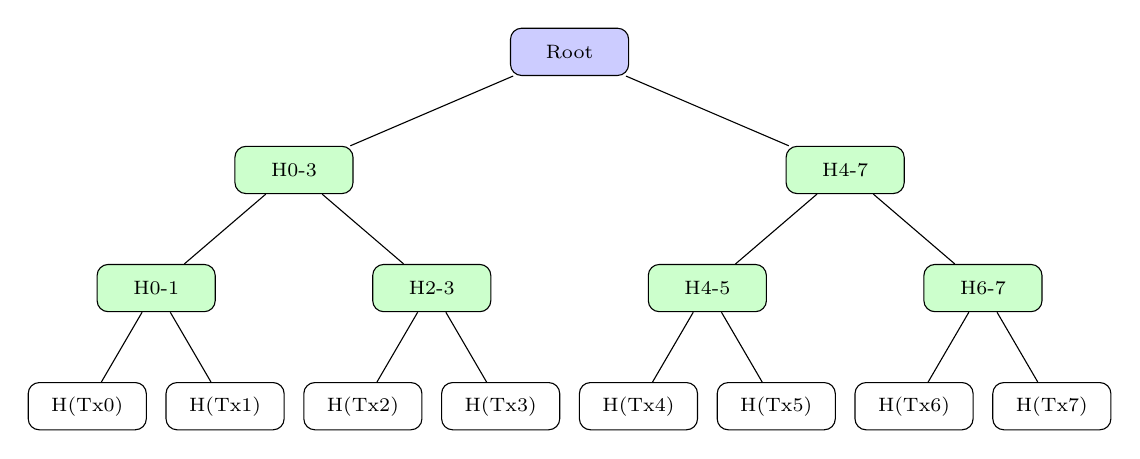
\begin{tikzpicture}[
				level distance=1.5cm,
				level 1/.style={sibling distance=7cm},
				level 2/.style={sibling distance=3.5cm},
				level 3/.style={sibling distance=1.75cm},
				every node/.style={rectangle, draw, rounded corners, minimum width=1.5cm, minimum height=0.6cm, font=\scriptsize}
			]
			\node[fill=blue!20] {Root}
			child {node[fill=green!20] {H0-3}
					child {node[fill=green!20] {H0-1}
							child {node {H(Tx0)}}
							child {node {H(Tx1)}}
						}
					child {node[fill=green!20] {H2-3}
							child {node {H(Tx2)}}
							child {node {H(Tx3)}}
						}
				}
			child {node[fill=green!20] {H4-7}
					child {node[fill=green!20] {H4-5}
							child {node {H(Tx4)}}
							child {node {H(Tx5)}}
						}
					child {node[fill=green!20] {H6-7}
							child {node {H(Tx6)}}
							child {node {H(Tx7)}}
						}
				};
		\end{tikzpicture}
	\end{center}
	\begin{center}
		\textbf{Blue = What goes in block header | Green = Intermediate nodes | White = Leaves}
	\end{center}
\end{frame}

\begin{frame}{How to build a Merkle tree: Step by step}
	\begin{columns}[c]
		\begin{column}{0.5\textwidth}
			\textbf{Start with transactions:}
			\begin{itemize}
				\item Hash each transaction
				\item These are the leaves
				\item Think: bottom of the tree
			\end{itemize}
			\vspace{0.5em}
			\textbf{Build upward:}
			\begin{enumerate}
				\item Pair adjacent hashes
				\item Concatenate them
				\item Hash the result
				\item This is the parent node
				\item Repeat until one hash left!
			\end{enumerate}
		\end{column}
		\begin{column}{0.5\textwidth}
			\textbf{Example with 4 transactions:}
			\begin{itemize}
				\item Level 0 (leaves):
				      \begin{itemize}
					      \item H(Tx0), H(Tx1)
					      \item H(Tx2), H(Tx3)
				      \end{itemize}
				\item Level 1:
				      \begin{itemize}
					      \item H01 = hash(H(Tx0) $\|$ H(Tx1))
					      \item H23 = hash(H(Tx2) $\|$ H(Tx3))
				      \end{itemize}
				\item Level 2 (root):
				      \begin{itemize}
					      \item Root = hash(H01 $\|$ H23)
				      \end{itemize}
			\end{itemize}
		\end{column}
	\end{columns}
\end{frame}

\begin{frame}{The power: Logarithmic proofs}
	\begin{center}
		\textbf{This is where Merkle trees shine!}
	\end{center}
	\vspace{0.5em}
	\begin{columns}[c]
		\begin{column}{0.5\textwidth}
			\textbf{To prove Tx2 is in the block:}
			\begin{itemize}
				\item Don't need all 8 transactions
				\item Only need the ``sibling path''
				\item Just 3 hashes:
				      \begin{enumerate}
					      \item H(Tx3) - sibling
					      \item H0-1 - uncle
					      \item H4-7 - aunt
				      \end{enumerate}
				\item Plus Tx2 itself
			\end{itemize}
		\end{column}
		\begin{column}{0.5\textwidth}
			\textbf{The math:}
			\begin{itemize}
				\item 8 txs: Need 3 hashes
				\item 1,024 txs: Need 10 hashes
				\item 1 million txs: Need 20 hashes
				\item Path length = $\log_2(n)$
			\end{itemize}
			\vspace{0.5em}
			\begin{exampleblock}{Incredible efficiency}
				Proof stays tiny even as block grows huge!
			\end{exampleblock}
		\end{column}
	\end{columns}
\end{frame}

\begin{frame}{Visualizing the proof path}
	\begin{center}
		\textbf{Proving Tx2 is in the block}
	\end{center}
	\begin{columns}[c]
		\begin{column}{0.5\textwidth}
			\begin{center}
				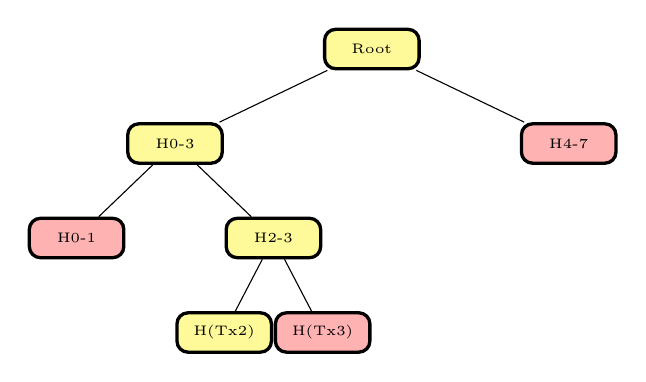
\begin{tikzpicture}[
						level distance=1.2cm,
						level 1/.style={sibling distance=5cm},
						level 2/.style={sibling distance=2.5cm},
						level 3/.style={sibling distance=1.25cm},
						every node/.style={rectangle, draw, rounded corners, minimum width=1.2cm, minimum height=0.5cm, font=\tiny}
					]
					\node[fill=yellow!40, very thick] {Root}
					child {node[fill=yellow!40, very thick] {H0-3}
							child {node[fill=red!30, very thick] {H0-1}}
							child {node[fill=yellow!40, very thick] {H2-3}
									child {node[fill=yellow!40, very thick] {H(Tx2)}}
									child {node[fill=red!30, very thick] {H(Tx3)}}
								}
						}
					child {node[fill=red!30, very thick] {H4-7}};
				\end{tikzpicture}
			\end{center}
		\end{column}
		\begin{column}{0.5\textwidth}
			\begin{itemize}
				\item \textbf{Yellow = Compute these}: Start with Tx2, hash upward
				\item \textbf{Red = Proof provides these}: Just 3 hashes needed!
			\end{itemize}
		\end{column}
	\end{columns}
\end{frame}

\begin{frame}{Step-by-step verification}
	\begin{columns}[c]
		\begin{column}{0.5\textwidth}
			\textbf{What verifier has:}
			\begin{itemize}
				\item Transaction Tx2
				\item Merkle proof: [H(Tx3), H0-1, H4-7]
				\item Block header with root
			\end{itemize}
			\vspace{0.5em}
			\textbf{What verifier does:}
			\begin{enumerate}
				\item Hash Tx2 \rightarrow\ H(Tx2)
				\item Combine with H(Tx3)
				\item Hash \rightarrow\ H2-3
				\item Combine with H0-1
				\item Hash \rightarrow\ H0-3
			\end{enumerate}
		\end{column}
		\begin{column}{0.5\textwidth}
			\begin{enumerate}
				\setcounter{enumi}{5}
				\item Combine with H4-7
				\item Hash \rightarrow\ Computed Root
				\item Compare with header
			\end{enumerate}
			\vspace{0.5em}
			\begin{alertblock}{If they match}
				Tx2 is definitely in the block! Can't fake this without breaking SHA-256.
			\end{alertblock}
			\vspace{0.5em}
			\textbf{Data transferred:}\\
			Tx2 + 3 hashes = \approx400 bytes\\
			Instead of 1 MB!
		\end{column}
	\end{columns}
\end{frame}

\begin{frame}{Where do Merkle proofs come from?}
	\begin{columns}[c]
		\begin{column}{0.5\textwidth}
			\textbf{The question:}
			\begin{itemize}
				\item You have the Merkle root
				\item You want to verify a transaction
				\item But you need sibling hashes
				\item Where do they come from?
			\end{itemize}
			\vspace{0.5em}
			\textbf{The answer:}
			\begin{itemize}
				\item \textbf{Full nodes have everything}\footnote{\url{https://learnmeabitcoin.com/technical/block/merkle-root/}}
				\item \textbf{They store the entire block}
				\item \textbf{Including all transactions}
				\item Can compute any proof
			\end{itemize}
		\end{column}
		\begin{column}{0.5\textwidth}
			\textbf{How full nodes generate proofs:}
			\begin{enumerate}
				\item Store all transactions in block
				\item Rebuild the Merkle tree
				\item Find transaction's position
				\item Walk up tree, collect siblings
				\item Return proof path
			\end{enumerate}
			\vspace{0.5em}
			\begin{alertblock}{Key point}
				Full nodes can generate proofs for any transaction because they have the complete block data!
			\end{alertblock}
		\end{column}
	\end{columns}
\end{frame}

\begin{frame}{Full node verification workflow}
	\begin{columns}[c]
		\begin{column}{0.5\textwidth}
			\textbf{When full node receives block:}
			\begin{enumerate}
				\item Download all transactions
				\item Build Merkle tree locally
				\item Compute root
				\item Compare with block header
				\item If match: block valid!
			\end{enumerate}
			\vspace{0.5em}
			\textbf{To verify specific transaction:}
			\begin{itemize}
				\item Already has full tree
				\item Extract sibling path
				\item Verify against root
			\end{itemize}
		\end{column}
		\begin{column}{0.5\textwidth}
			\textbf{Example scenario:}
			\begin{itemize}
				\item Your wallet queries your full node
				\item ``Is transaction X in block 850000?''
				\item Full node:
				      \begin{enumerate}
					      \item Has block 850000 stored
					      \item Locates transaction X
					      \item Generates proof path
					      \item Returns proof to wallet
				      \end{enumerate}
			\end{itemize}
			\vspace{0.5em}
			\begin{exampleblock}{Trust model}
				Full nodes trust no one - they verify everything themselves!
			\end{exampleblock}
		\end{column}
	\end{columns}
\end{frame}

\begin{frame}{SPV: Simplified Payment Verification}
	\begin{columns}[c]
		\begin{column}{0.5\textwidth}
			\textbf{Full node:}
			\begin{itemize}
				\item Downloads everything
				\item Validates all transactions
				\item Stores full blockchain
				\item Requirement: \approx500 GB
				\item Time to sync: Days
			\end{itemize}
			\vspace{0.5em}
			\textbf{Not practical for most users!}
		\end{column}
		\begin{column}{0.5\textwidth}
			\textbf{SPV client:}
			\begin{itemize}
				\item Downloads only headers
				\item 80 bytes $\times$ 850K blocks
				\item Requirement: \approx60 MB
				\item Syncs in minutes
				\item Requests Merkle proofs as needed
			\end{itemize}
			\vspace{0.5em}
			\begin{exampleblock}{8000$\times$ smaller!}
				This is why Bitcoin works on phones!
			\end{exampleblock}
		\end{column}
	\end{columns}
\end{frame}

\begin{frame}{How SPV wallets work}
	\begin{columns}[c]
		\begin{column}{0.5\textwidth}
			\textbf{Setup:}
			\begin{enumerate}
				\item Download all block headers
				\item Verify PoW chain
				\item Store locally (tiny!)
				\item Now ready
			\end{enumerate}
			\vspace{0.5em}
			\textbf{When payment arrives:}
			\begin{enumerate}
				\item Peer says: ``You got paid!''
				\item SPV wallet: ``Prove it''
				\item Peer sends Merkle proof
				\item Wallet verifies against header
			\end{enumerate}
		\end{column}
		\begin{column}{0.5\textwidth}
			\textbf{Security:}
			\begin{itemize}
				\item Can verify inclusion
				\item Can't verify validity
				      \begin{itemize}
					      \item Trust PoW majority
					      \item Full nodes reject invalid
				      \end{itemize}
				\item Wait for confirmations
				\item Connect to multiple peers
			\end{itemize}
			\vspace{0.5em}
			\begin{alertblock}{Trade-off}
				Less security than full node, but good enough for most use cases
			\end{alertblock}
		\end{column}
	\end{columns}
\end{frame}

\begin{frame}{Handling odd transaction counts}
	\begin{columns}[c]
		\begin{column}{0.5\textwidth}
			\textbf{The problem:}
			\begin{itemize}
				\item Binary trees need pairs
				\item What if 5 transactions?
				\item Can't pair the last one
			\end{itemize}
			\vspace{0.5em}
			\textbf{Bitcoin's solution:}
			\begin{itemize}
				\item Duplicate the last hash
				\item Tx4's hash appears twice
				\item Now we have 6 leaves
				\item Tree is complete!
			\end{itemize}
		\end{column}
		\begin{column}{0.5\textwidth}
			\textbf{Important distinction:}
			\begin{itemize}
				\item Duplicate the \textit{hash}
				\item NOT the transaction itself
				\item Transaction only in block once
				\item Prevents weird edge cases
			\end{itemize}
			\vspace{0.5em}
			\begin{exampleblock}{Visual}
				Leaves: H(Tx0), H(Tx1), H(Tx2), H(Tx3), H(Tx4), \textcolor{red}{H(Tx4)}
			\end{exampleblock}
		\end{column}
	\end{columns}
\end{frame}

\begin{frame}{Why Merkle trees are brilliant}
	\begin{columns}[c]
		\begin{column}{0.5\textwidth}
			\textbf{Efficiency:}
			\begin{itemize}
				\item Logarithmic proof size
				\item Constant verification time
				\item Enables light clients
				\item Mobile-friendly
			\end{itemize}
			\vspace{0.5em}
			\textbf{Security:}
			\begin{itemize}
				\item Tamper-evident
				\item Change any tx \rightarrow\ root changes
				\item Based on collision resistance
				\item Strong as SHA-256
			\end{itemize}
		\end{column}
		\begin{column}{0.5\textwidth}
			\textbf{Privacy:}
			\begin{itemize}
				\item Prove one transaction
				\item Don't reveal others
				\item Selective disclosure
			\end{itemize}
			\vspace{0.5em}
			\textbf{Storage:}
			\begin{itemize}
				\item Old nodes can prune
				\item Keep headers only
				\item Serve proofs on demand
			\end{itemize}
			\vspace{0.5em}
			\begin{alertblock}{Fundamental primitive}
				Merkle trees make Bitcoin scalable!
			\end{alertblock}
		\end{column}
	\end{columns}
\end{frame}

\begin{frame}{Security properties in detail}
	\begin{columns}[c]
		\begin{column}{0.5\textwidth}
			\textbf{Tamper evidence:}
			\begin{itemize}
				\item Modify any transaction
				\item Its hash changes
				\item Parent hash changes
				\item Propagates to root
				\item Root in header changes
				\item Breaks PoW!
			\end{itemize}
			\vspace{0.5em}
			\textbf{Collision resistance:}
			\begin{itemize}
				\item From SHA-256
				\item Can't find two transactions with same hash
			\end{itemize}
		\end{column}
		\begin{column}{0.5\textwidth}
			\textbf{Commitment:}
			\begin{itemize}
				\item Root commits to:
				      \begin{itemize}
					      \item All transactions
					      \item Their content
					      \item Their order
				      \end{itemize}
				\item Can't change after PoW
			\end{itemize}
			\vspace{0.5em}
			\textbf{Second preimage resistance:}
			\begin{itemize}
				\item Can't find different tx with same proof path
				\item Would need to break hash function
			\end{itemize}
		\end{column}
	\end{columns}
\end{frame}

\begin{frame}{Potential attacks and mitigations}
	\begin{columns}[c]
		\begin{column}{0.5\textwidth}
			\textbf{Attack scenario:}
			\begin{itemize}
				\item Malicious miner
				\item Includes invalid transaction
				\item Valid Merkle proof though!
				\item SPV client can't tell
			\end{itemize}
			\vspace{0.5em}
			\textbf{Why it's hard:}
			\begin{itemize}
				\item Full nodes reject invalid blocks
				\item Miner loses block reward
				\item Economic disincentive
				\item Need 51\% to succeed
			\end{itemize}
		\end{column}
		\begin{column}{0.5\textwidth}
			\textbf{SPV best practices:}
			\begin{itemize}
				\item Connect to multiple peers
				\item Wait for confirmations
				\item Check PoW chain is longest
				\item For large amounts: run full node
			\end{itemize}
			\vspace{0.5em}
			\begin{alertblock}{Security model}
				SPV trusts that majority hashpower is honest - same as full nodes!
			\end{alertblock}
		\end{column}
	\end{columns}
\end{frame}

\begin{frame}{Beyond Bitcoin: Merkle trees everywhere}
	\begin{columns}[c]
		\begin{column}{0.5\textwidth}
			\textbf{Other blockchains:}
			\begin{itemize}
				\item Ethereum: 3 Merkle trees per block
				      \begin{itemize}
					      \item Transactions
					      \item Receipts
					      \item State (accounts)
				      \end{itemize}
				\item Most cryptocurrencies use them
			\end{itemize}
			\vspace{0.5em}
			\textbf{Beyond crypto:}
			\begin{itemize}
				\item Git version control
				\item IPFS content addressing
				\item Certificate Transparency
			\end{itemize}
		\end{column}
		\begin{column}{0.5\textwidth}
			\textbf{We've seen them before!}
			\begin{itemize}
				\item MLS (Secure Messaging)
				\item TreeKEM for group keys
			\end{itemize}
			\vspace{0.5em}
			\textbf{Future variants:}
			\begin{itemize}
				\item Verkle trees (smaller proofs)
				\item Sparse Merkle trees (state)
				\item Merkle-sum trees (amounts)
			\end{itemize}
		\end{column}
	\end{columns}
	\vspace{0.25cm}
	\begin{exampleblock}{Universal primitive}
		Merkle trees: A fundamental tool for authenticated data structures
	\end{exampleblock}
\end{frame}

\begin{frame}{Example: Git is a blockchain!}
	\begin{columns}[c]
		\begin{column}{0.5\textwidth}
			\textbf{Git commits are blocks:}
			\begin{itemize}
				\item Each commit has:
				      \begin{itemize}
					      \item Content (like transactions)
					      \item Timestamp
					      \item Hash of parent commit
					      \item Author signature
				      \end{itemize}
				\item Forms a chain back to initial commit
				\item Change any commit \rightarrow\ all subsequent hashes change
			\end{itemize}
		\end{column}
		\begin{column}{0.5\textwidth}
			\textbf{Key differences:}
			\begin{itemize}
				\item Git: Centralized (GitHub)
				\item Bitcoin: Decentralized (P2P)
				\item Git: No proof-of-work
				\item Bitcoin: Mining required
				\item Git: Trust repository owner
				\item Bitcoin: Trust no one
			\end{itemize}
			\vspace{0.5em}
			\begin{exampleblock}{Same primitive}
				Both use Merkle trees and hash chains for tamper-evident history!
			\end{exampleblock}
		\end{column}
	\end{columns}
\end{frame}

\section{Ethereum and Smart Contracts}

\begin{frame}{Bitcoin's limitation: Just digital cash}
	\begin{columns}[c]
		\begin{column}{0.5\textwidth}
			\textbf{Bitcoin can only:}
			\begin{itemize}
				\item Send coins from A to B
				\item Simple spending conditions
				\item No loops or complex logic
			\end{itemize}
			\vspace{0.5em}
			\textbf{Why?}
			\begin{itemize}
				\item Intentionally limited scripting
				\item Security through simplicity
				\item One job: be money
			\end{itemize}
		\end{column}
		\begin{column}{0.5\textwidth}
			\textbf{What if we want more?}
			\begin{itemize}
				\item Automated loans
				\item Decentralized exchanges
				\item Digital property
				\item Autonomous organizations
			\end{itemize}
			\vspace{0.5em}
			\begin{exampleblock}{The vision}
				Programmable money with arbitrary logic!
			\end{exampleblock}
		\end{column}
	\end{columns}
\end{frame}

\begin{frame}{Ethereum: Bitcoin + programming}
	\begin{center}
		\textbf{What if the blockchain could run any program?}
	\end{center}
	\vspace{0.5em}
	\begin{columns}[c]
		\begin{column}{0.5\textwidth}
			\textbf{The idea (2013):}
			\begin{itemize}
				\item Vitalik Buterin's insight
				\item Blockchain as ``world computer''
				\item Store code, not just transactions
				\item Every node executes the code
			\end{itemize}
		\end{column}
		\begin{column}{0.5\textwidth}
			\textbf{Key innovation:}
			\begin{itemize}
				\item Turing-complete language
				\item Persistent state storage
				\item Global consensus on computation
				\item Anyone can deploy code
			\end{itemize}
			\vspace{0.5em}
			\begin{alertblock}{Result}
				``Smart contracts'' - code that runs trustlessly on the blockchain
			\end{alertblock}
		\end{column}
	\end{columns}
\end{frame}

\begin{frame}{From Bitcoin to Ethereum}
	\begin{columns}[c]
		\begin{column}{0.5\textwidth}
			\textbf{Bitcoin:}
			\begin{itemize}
				\item UTXO model (like cash)
				\item Limited scripting
				\item Tracks coin ownership
				\item Simple state transitions
			\end{itemize}
		\end{column}
		\begin{column}{0.5\textwidth}
			\textbf{Ethereum:}
			\begin{itemize}
				\item Account model (like bank accounts)
				\item Full programming
				\item Tracks balances + code + data
				\item Complex state machine
			\end{itemize}
		\end{column}
	\end{columns}
	\vspace{1em}
	\begin{center}
		\textbf{Every transaction can trigger arbitrary code execution}
	\end{center}
\end{frame}

\subsection{Smart Contracts}

\begin{frame}{What are smart contracts?}
	\begin{columns}[c]
		\begin{column}{0.5\textwidth}
			\textbf{The vending machine:}
			\begin{itemize}
				\item Insert \$1.50 \rightarrow\ get soda
				\item Rules built into machine
				\item No human intermediary
				\item Can't cheat the machine
			\end{itemize}
		\end{column}
		\begin{column}{0.5\textwidth}
			\textbf{Smart contracts:}
			\begin{itemize}
				\item Code on blockchain
				\item Rules in the code
				\item Executes automatically
				\item Can't be stopped or changed
			\end{itemize}
			\vspace{0.5em}
			\begin{exampleblock}{Four key properties}
				Immutable • Deterministic • Autonomous • Transparent
			\end{exampleblock}
		\end{column}
	\end{columns}
\end{frame}

\begin{frame}[fragile]{Your first smart contract}
	\begin{columns}[c]
		\begin{column}{0.6\textwidth}
			\scriptsize
			\begin{verbatim}
pragma solidity ^0.8.0;

contract SimpleStorage {
  uint256 public number;

  function store(uint256 _num) public {
    number = _num;
  }

  function retrieve() public view returns (uint256) {
    return number;
  }
}
\end{verbatim}
		\end{column}
		\begin{column}{0.4\textwidth}
			\textbf{What this does:}
			\begin{itemize}
				\item Stores one number
				\item Anyone can update it
				\item Anyone can read it
				\item Lives forever on blockchain
			\end{itemize}
			\vspace{0.5em}
			\textbf{Language: Solidity}
			\begin{itemize}
				\item Like JavaScript + types
				\item Compiles to bytecode
				\item Runs on EVM
			\end{itemize}
		\end{column}
	\end{columns}
\end{frame}

\begin{frame}{How smart contracts work: The lifecycle}
	\begin{columns}[c]
		\begin{column}{0.5\textwidth}
			\textbf{1. Deployment:}
			\begin{itemize}
				\item Write code (Solidity)
				\item Compile to bytecode
				\item Send deployment transaction
				\item Contract gets address
				\item Now lives on blockchain!
			\end{itemize}
		\end{column}
		\begin{column}{0.5\textwidth}
			\textbf{2. Interaction:}
			\begin{itemize}
				\item Send transaction to contract
				\item Call specific function
				\item All nodes execute code
				\item State changes recorded
				\item Everyone sees same result
			\end{itemize}
		\end{column}
	\end{columns}
	\vspace{1em}
	\begin{alertblock}{Key insight}
		Once deployed, the code is \textbf{law}. No one can change it, not even the creator!
	\end{alertblock}
\end{frame}

\begin{frame}{The gas mechanism: Paying for computation}
	\begin{columns}[c]
		\begin{column}{0.5\textwidth}
			\textbf{Problem:}
			\begin{itemize}
				\item What stops infinite loops?
				\item What prevents spam?
				\item How to price CPU time?
			\end{itemize}
			\vspace{0.5em}
			\textbf{Solution: Gas}
			\begin{itemize}
				\item Every operation costs gas
				\item Storage most expensive
				\item Simple math cheap
				\item User pays for execution
			\end{itemize}
		\end{column}
		\begin{column}{0.5\textwidth}
			\textbf{Gas prices:}
			\begin{itemize}
				\item ADD: 3 gas
				\item Multiply: 5 gas
				\item Store data: 20,000 gas
			\end{itemize}
			\vspace{0.5em}
			\textbf{How it works:}
			\begin{itemize}
				\item Set gas limit \& price
				\item Fee = gas used $\times$ price
				\item Out of gas? Reverts!
			\end{itemize}
			\vspace{0.5em}
			\begin{exampleblock}{Brilliance}
				Solves halting problem with economics!
			\end{exampleblock}
		\end{column}
	\end{columns}
\end{frame}

\begin{frame}[fragile]{A real example: Simple token}
	\scriptsize
	\begin{verbatim}
contract SimpleToken {
  mapping(address => uint256) public balances;

  constructor(uint256 initialSupply) {
    balances[msg.sender] = initialSupply;
  }

  function transfer(address to, uint256 amount) public returns (bool) {
    require(balances[msg.sender] >= amount, "Insufficient balance");
    balances[msg.sender] -= amount;
    balances[to] += amount;
    return true;
  }
}
		\end{verbatim}
	\vspace{0.5em}
	\textbf{Key concepts:} \texttt{msg.sender} (who called this?), \texttt{mapping} (key-value storage), \texttt{require} (check conditions)
\end{frame}

\begin{frame}{The DAO hack: When code goes wrong}
	\begin{columns}[c]
		\begin{column}{0.5\textwidth}
			\textbf{June 2016:}
			\begin{itemize}
				\item The DAO raises \$150M
				\item Largest crowdfund ever
				\item Decentralized VC fund
				\item All controlled by code
			\end{itemize}
			\vspace{0.5em}
			\textbf{The attack:}
			\begin{itemize}
				\item Reentrancy vulnerability
				\item Withdraw function flawed
				\item \$60M stolen in hours
			\end{itemize}
		\end{column}
		\begin{column}{0.5\textwidth}
			\textbf{What went wrong:}
			\begin{enumerate}
				\item Call withdraw()
				\item Contract sends ETH
				\item Before updating balance...
				\item Attacker calls withdraw again!
				\item Repeat until drained
			\end{enumerate}
			\vspace{0.5em}
			\begin{alertblock}{Lesson}
				Code is law... but bugs are expensive! Led to Ethereum hard fork.
			\end{alertblock}
		\end{column}
	\end{columns}
\end{frame}

\begin{frame}{Security matters: Common vulnerabilities}
	\begin{columns}[c]
		\begin{column}{0.5\textwidth}
			\textbf{Top threats:}
			\begin{itemize}
				\item \textbf{Reentrancy}: Like The DAO
				\item \textbf{Access control}: Who can call what?
				\item \textbf{Integer issues}: Over/underflow
				\item \textbf{Front-running}: Seeing txs before they execute
			\end{itemize}
		\end{column}
		\begin{column}{0.5\textwidth}
			\textbf{Best practices:}
			\begin{itemize}
				\item Use OpenZeppelin libraries
				\item Check-Effects-Interactions pattern
				\item Comprehensive testing
				\item Professional audits
				\item Bug bounties
			\end{itemize}
			\vspace{0.5em}
			\begin{exampleblock}{Remember}
				Can't patch code after deployment!
			\end{exampleblock}
		\end{column}
	\end{columns}
\end{frame}

\begin{frame}{Real-world applications}
	\begin{columns}[c]
		\begin{column}{0.5\textwidth}
			\textbf{DeFi (Decentralized Finance):}
			\begin{itemize}
				\item Uniswap: Token swaps
				\item Aave: Lending/borrowing
				\item MakerDAO: Stablecoin
			\end{itemize}
			\vspace{0.5em}
			\textbf{NFTs:}
			\begin{itemize}
				\item Digital art ownership
				\item Gaming items
				\item Collectibles
			\end{itemize}
		\end{column}
		\begin{column}{0.5\textwidth}
			\textbf{Other uses:}
			\begin{itemize}
				\item DAOs: Decentralized orgs
				\item ENS: Domain names
				\item Multi-sig wallets
				\item Prediction markets
			\end{itemize}
			\vspace{0.5em}
			\begin{alertblock}{The impact}
				\$50B+ locked in DeFi protocols!
			\end{alertblock}
		\end{column}
	\end{columns}
\end{frame}

\subsection{Proof of Stake: The Merge}

\begin{frame}{The energy problem}
	\begin{columns}[c]
		\begin{column}{0.5\textwidth}
			\textbf{Ethereum's PoW:}
			\begin{itemize}
				\item Like Bitcoin mining
				\item Massive energy use
				\item 78 TWh/year
				\item More than Austria!
			\end{itemize}
			\vspace{0.5em}
			\textbf{The question:}
			\begin{itemize}
				\item Can we secure network...
				\item Without burning energy?
				\item Still stay decentralized?
			\end{itemize}
		\end{column}
		\begin{column}{0.5\textwidth}
			\textbf{Proof of Stake idea:}
			\begin{itemize}
				\item Replace miners with validators
				\item Stake ETH as collateral
				\item Get randomly selected
				\item Misbehave? Lose your stake!
			\end{itemize}
			\vspace{0.5em}
			\begin{exampleblock}{Core insight}
				Economic security instead of energy security
			\end{exampleblock}
		\end{column}
	\end{columns}
\end{frame}

\begin{frame}{The Merge: September 2022}
	\begin{center}
		\textbf{One of the most ambitious upgrades in tech history}
	\end{center}
	\vspace{0.5em}
	\begin{columns}[c]
		\begin{column}{0.5\textwidth}
			\textbf{What happened:}
			\begin{itemize}
				\item Swapped consensus engine
				\item While network was running
				\item \$200B+ at stake
				\item Zero downtime
				\item Like changing plane engines mid-flight!
			\end{itemize}
		\end{column}
		\begin{column}{0.5\textwidth}
			\textbf{Results:}
			\begin{itemize}
				\item 99.95\% energy reduction
				\item 900K+ validators
				\item \$40B+ staked
				\item 13-minute finality
				\item Network more secure than ever
			\end{itemize}
		\end{column}
	\end{columns}
	\vspace{0.5em}
	\begin{center}
		\textbf{From 13,000 households worth of energy to just 10}
	\end{center}
\end{frame}

\begin{frame}{How PoS works}
	\begin{columns}[c]
		\begin{column}{0.5\textwidth}
			\textbf{Become a validator:}
			\begin{itemize}
				\item Stake 32 ETH (\approx\$100K)
				\item Run validator software
				\item Stay online
				\item Act honestly
			\end{itemize}
			\vspace{0.5em}
			\textbf{Rewards:}
			\begin{itemize}
				\item \approx4-5\% annual yield
				\item Block proposals
				\item Attestations
			\end{itemize}
		\end{column}
		\begin{column}{0.5\textwidth}
			\textbf{Penalties:}
			\begin{itemize}
				\item Offline? Small penalties
				\item Double-sign? Slashed!
				\item Lose stake + ejected
			\end{itemize}
			\vspace{0.5em}
			\begin{alertblock}{Skin in the game}
				Can't fake having stake. Attack costs real money you'll lose!
			\end{alertblock}
		\end{column}
	\end{columns}
\end{frame}

\subsection{Scaling: Layer 2s}

\begin{frame}{The blockchain trilemma}
	\begin{center}
		\textbf{Pick any two:}
	\end{center}
	\vspace{0.5em}
	\begin{columns}[c]
		\begin{column}{0.33\textwidth}
			\centering
			\textbf{Decentralization}\\
			Many validators
		\end{column}
		\begin{column}{0.33\textwidth}
			\centering
			\textbf{Security}\\
			Attack-resistant
		\end{column}
		\begin{column}{0.33\textwidth}
			\centering
			\textbf{Scalability}\\
			High throughput
		\end{column}
	\end{columns}
	\vspace{1em}
	\begin{center}
		\textbf{The problem:}\\
		Ethereum: 15 TPS\\
		Visa: 65,000 TPS\\
		Gap: 4,000$\times$
	\end{center}
	\vspace{0.5em}
	\begin{alertblock}{Why so slow?}
		Every node processes every transaction. Can't just use bigger servers!
	\end{alertblock}
\end{frame}

\begin{frame}{Layer 2: The solution}
	\begin{columns}[c]
		\begin{column}{0.5\textwidth}
			\textbf{Key insight:}
			\begin{itemize}
				\item Not every node needs to execute every transaction
				\item Execute elsewhere
				\item Post results to Ethereum
				\item Prove correctness
			\end{itemize}
			\vspace{0.5em}
			\textbf{L1 (Ethereum):}
			\begin{itemize}
				\item Security layer
				\item Final settlement
				\item Data availability
			\end{itemize}
		\end{column}
		\begin{column}{0.5\textwidth}
			\textbf{L2 (Rollups):}
			\begin{itemize}
				\item Execute transactions
				\item Much cheaper
				\item Much faster
				\item Inherit L1 security
			\end{itemize}
			\vspace{0.5em}
			\begin{exampleblock}{The result}
				100x cheaper fees, 100x higher throughput, same security!
			\end{exampleblock}
		\end{column}
	\end{columns}
\end{frame}

\begin{frame}{Two types of rollups}
	\begin{columns}[c]
		\begin{column}{0.5\textwidth}
			\textbf{Optimistic Rollups:}
			\begin{itemize}
				\item Assume transactions valid
				\item 7-day challenge period
				\item Anyone can prove fraud
				\item If fraud found, rollback
			\end{itemize}
			\vspace{0.5em}
			\textbf{Examples:}
			\begin{itemize}
				\item Arbitrum (\$15B TVL)
				\item Optimism (\$7B TVL)
				\item Base (Coinbase's L2)
			\end{itemize}
		\end{column}
		\begin{column}{0.5\textwidth}
			\textbf{ZK Rollups:}
			\begin{itemize}
				\item Cryptographic validity proofs
				\item Instant finality
				\item No waiting period
				\item Math proves correctness
			\end{itemize}
			\vspace{0.5em}
			\textbf{Examples:}
			\begin{itemize}
				\item zkSync
				\item StarkNet
				\item Polygon zkEVM
			\end{itemize}
		\end{column}
	\end{columns}
	\vspace{0.5em}
	\begin{center}
		\textbf{Both inherit Ethereum's security. Different trade-offs on speed vs complexity.}
	\end{center}
\end{frame}

\begin{frame}{The L2 revolution}
	\begin{columns}[c]
		\begin{column}{0.5\textwidth}
			\textbf{The numbers:}
			\begin{itemize}
				\item L2s process 5-10$\times$ more than Ethereum
				\item Fees 10-100$\times$ cheaper
				\item 50+ L2s live or in development
				\item Transaction: \$0.10 vs \$10
			\end{itemize}
		\end{column}
		\begin{column}{0.5\textwidth}
			\textbf{Why this matters:}
			\begin{itemize}
				\item Makes crypto actually usable
				\item Enables mass adoption
				\item Preserves decentralization
				\item No compromise on security
			\end{itemize}
			\vspace{0.5em}
			\begin{exampleblock}{The future}
				Ethereum = settlement layer\\
				L2s = execution layer\\
				Users mostly interact with L2s
			\end{exampleblock}
		\end{column}
	\end{columns}
\end{frame}

\begin{frame}{Challenges ahead}
	\begin{columns}[c]
		\begin{column}{0.5\textwidth}
			\textbf{Current issues:}
			\begin{itemize}
				\item Fragmentation (many L2s)
				\item Moving between L2s hard
				\item Centralized sequencers
				\item Complex for users
			\end{itemize}
		\end{column}
		\begin{column}{0.5\textwidth}
			\textbf{Being solved:}
			\begin{itemize}
				\item Shared sequencers
				\item Fast bridges
				\item Better UX
				\item Decentralization roadmaps
			\end{itemize}
		\end{column}
	\end{columns}
	\vspace{1em}
	\begin{center}
		\textbf{The ecosystem is evolving fast. L2s are the path to scaling Ethereum while preserving what makes it special.}
	\end{center}
\end{frame}

\begin{frame}[plain]
	\titlepage
\end{frame}
\end{document}
